\subsection{Connecting homomorphisms and exact sequences}

Let M be an A-module. Recall that for every A-module N, we defined in the preceding number an isomorphism of k-modules

\[
\varphi_ {\mathbf {M}} (\mathbf {N}): \mathrm{H} (\operatorname{Homgr} _ {\mathbf {A}} (\mathrm{L} (\mathbf {M}), \mathbf {N})) \rightarrow \operatorname{Ext} _ {\mathbf {A}} (\mathbf {M}, \mathbf {N}).
\]

Let

\[
0 \to \mathbf {N} ^ {\prime} \xrightarrow {u} \mathbf {N} \xrightarrow {v} \mathbf {N} ^ {\prime \prime} \to 0\tag{$(\mathcal{E})$}
\]

an exact sequence of A-modules; the sequence of k-complexes

\[
\begin{array}{r l} \left(\mathbf {M} ^ {\mathcal {E}}\right) & 0 \longrightarrow \operatorname{Homgr} _ {\mathbf {A}} (\mathrm{L} (\mathrm{M}), \mathrm{N} ^ {\prime}) \xrightarrow {\operatorname{Homgr} (1 , u)} \operatorname{Homgr} _ {\mathbf {A}} (\mathrm{L} (\mathrm{M}), \mathrm{N}) \\ & \xrightarrow {\operatorname{Homgr} (1 , v)} \operatorname{Homgr} _ {\mathbf {A}} (\mathrm{L} (\mathrm{M}), \mathrm{N} ^ {\prime \prime}) \longrightarrow 0 \end{array}
\]

is then exact (X, p. 83, prop. 2, a)), i.e.

\[
\partial_ {(\mathbf {M} ^ {\mathcal {E}})}: \mathrm{H} (\operatorname{Homgr} _ {\mathbf {A}} (\mathrm{L} (\mathbf {M}), \mathrm{N} ^ {\prime \prime})) \rightarrow \mathrm{H} (\operatorname{Homgr} _ {\mathbf {A}} (\mathrm{L} (\mathbf {M}), \mathrm{N} ^ {\prime}))
\]

the corresponding connecting homomorphism (X, p. 29).

DEFINITION 2. --- A connecting homomorphism of extension modules relative to the module M and the exact sequence (\(\mathcal{E}\)) is called the composite homomorphism

\[
\delta (\mathbf {M}, \mathcal {E}) = \varphi_ {\mathbf {M}} (\mathbf {N} ^ {\prime}) \circ \partial_ {(\mathbf {M} ^ {\mathcal {E}})} \circ \varphi_ {\mathbf {M}} (\mathbf {N} ^ {\prime \prime}) ^ {- 1}: \operatorname{Ext} _ {\mathbf {A}} (\mathbf {M}, \mathbf {N} ^ {\prime \prime}) \rightarrow \operatorname{Ext} _ {\mathbf {A}} (\mathbf {M}, \mathbf {N} ^ {\prime}).
\]

This is a \(k\) -graded homomorphism of ascending degree 1, whose homogeneous components are denoted \(\delta^n (\mathbf{M},\mathcal{E})\colon \mathrm{Ext}_{\mathbf{A}}^{n}(\mathbf{M},\mathbf{N}^{\prime \prime})\to \mathrm{Ext}_{\mathbf{A}}^{n + 1}(\mathbf{M},\mathbf{N}^{\prime})\) .

THEOREM 1. --- The right-unbounded sequence of homomorphisms of k-modules

\[
\begin{array}{r l} 0 & \xrightarrow {\quad} \mathrm{Hom} _ {A} (M, N ^ {\prime}) \xrightarrow {\mathrm{Hom} (1 , u)} \mathrm{Hom} _ {A} (M, N) \xrightarrow {\mathrm{Hom} (1 , v)} \mathrm{Hom} _ {A} (M, N ^ {\prime \prime}) \\ & \xrightarrow {\delta (M , \mathcal {E})} \mathrm{Ext} _ {A} ^ {1} (M, N ^ {\prime}) \to \dots \xrightarrow {\delta^ {n - 1} (M , \mathcal {E})} \mathrm{Ext} _ {A} ^ {n} (M, N ^ {\prime}) \xrightarrow {\mathrm{Ext} ^ {n} (1 , u)} \mathrm{Ext} _ {A} ^ {n} (M, N) \\ & \xrightarrow {\mathrm{Ext} ^ {n} (1 , v)} \mathrm{Ext} _ {A} ^ {n} (M, N ^ {\prime \prime}) \xrightarrow {\delta^ {n} (M , \mathcal {E})} \mathrm{Ext} _ {A} ^ {n + 1} (M, N ^ {\prime}) \to \dots \end{array}
\]

is exact.

Consider indeed the diagram on page X. 91.

It is commutative by Remark 3 of X, p. 88 and Def. 2; moreover, the bottom row is exact (X, p. 30, Th. 1), and the vertical arrows are bijective (X, p. 88, prop. 5).

COROLLARY. --- If Ext \(_{A}^{1}\) (M, N') = 0, the sequence

\[
0 \longrightarrow \operatorname{Hom} _ {\mathbf {A}} (\mathrm{M}, \mathrm{N} ^ {\prime}) \xrightarrow {\operatorname{Hom} (1 , u)} \operatorname{Hom} _ {\mathbf {A}} (\mathrm{M}, \mathrm{N}) \xrightarrow {\operatorname{Hom} (1 , v)} \operatorname{Hom} _ {\mathbf {A}} (\mathrm{M}, \mathrm{N} ^ {\prime \prime}) \longrightarrow 0
\]

is exact.

PROPOSITION 8. --- Let \(f: \mathbf{M}_{1} \to \mathbf{M}\) be a homomorphism of A-modules and

\[
0 \longrightarrow \mathbf {N} ^ {\prime} \stackrel {u} {\longrightarrow} \mathbf {N} \stackrel {v} {\longrightarrow} \mathbf {N} ^ {\prime \prime} \longrightarrow 0\tag{$(\mathcal{E})$}
\]

\[
g ^ {\prime} \Big \downarrow \qquad \qquad g \Big \downarrow \qquad \qquad g ^ {\prime \prime} \Big \downarrow
\]

\[
0 \longrightarrow \mathrm{N} _ {1} ^ {\prime} \stackrel {u _ {1}} {\longrightarrow} \mathrm{N} _ {1} \stackrel {v _ {1}} {\longrightarrow} \mathrm{N} _ {1} ^ {\prime \prime} \longrightarrow 0\tag{$(\mathcal{E}_1)$}
\]

\pandocbounded{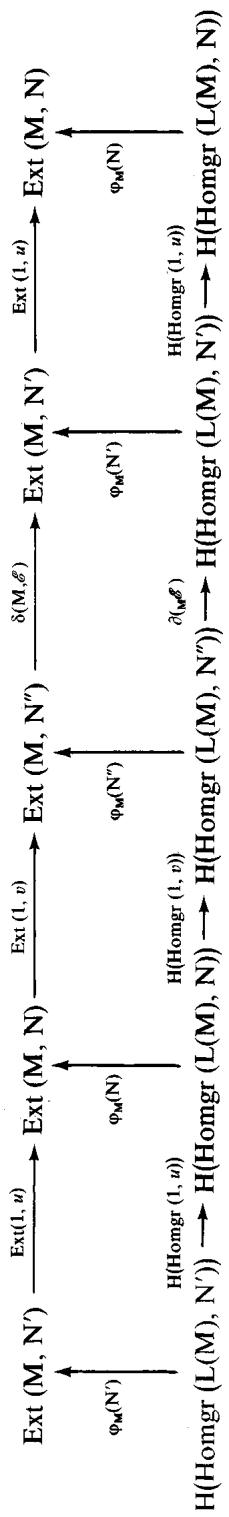
\includegraphics[keepaspectratio]{images/part001_97747f10.jpg}}

a commutative diagram of A-modules with exact rows. The diagram of k-modules

\[
\begin{array}{c} \operatorname{Ext} _ {\mathbf {A}} (\mathbf {M}, \mathbf {N} ^ {\prime \prime}) \xrightarrow {\delta (\mathbf {M} , \mathcal {E})} \operatorname{Ext} _ {\mathbf {A}} (\mathbf {M}, \mathbf {N} ^ {\prime}) \\ \operatorname{Ext} (f, g ^ {\prime \prime}) \Big | _ {\downarrow} \qquad \qquad \qquad \qquad \qquad \qquad \qquad \qquad \qquad \qquad \qquad \qquad \qquad \qquad \qquad \qquad \qquad \qquad \qquad \qquad \qquad \qquad \qquad \qquad \qquad \qquad \qquad \qquad \qquad \qquad \qquad \qquad \qquad \qquad \\ \operatorname{Ext} _ {\mathbf {A}} (\mathbf {M} _ {1}, \mathbf {N} _ {1} ^ {\prime \prime}) \xrightarrow {\delta (\mathbf {M} , \mathcal {E} _ {1})} \operatorname{Ext} _ {\mathbf {A}} (\mathbf {M} _ {1}, \mathbf {N} _ {1} ^ {\prime}) \end{array}
\]

is commutative.

This follows from X, p. 31, prop. 2 applied to the commutative diagram.

\[
\begin{array}{l} 0 \xrightarrow {\operatorname{Homgr} _ {A} (L (M) , N ^ {\prime})} \xrightarrow {\operatorname{Homgr} _ {A} (L (M) , N)} \xrightarrow {\operatorname{Homgr} _ {A} (L (M) , N ^ {\prime \prime})} 0 \\ \operatorname{Homgr} (L (f), g ^ {\prime}) \Big | _ {\downarrow} \quad \operatorname{Homgr} (1, u ^ {\prime}) \quad \Big | _ {\downarrow} \quad \operatorname{Homgr} (L (f), g) \quad \Big | _ {\downarrow} \quad \operatorname{Homgr} (L (f), g ^ {\prime \prime}) \\ 0 \xrightarrow {\operatorname{Homgr} _ {A} (L (M _ {1}) , N _ {1} ^ {\prime})} \xrightarrow {\operatorname{Homgr} _ {A} (L (M _ {1}) , N _ {1})} \xrightarrow {\operatorname{Homgr} _ {A} (L (M _ {1}) , N _ {1} ^ {\prime \prime})} 0 \end{array}
\]

Let N be an A-module, and

\[
0 \rightarrow \mathbf {M} ^ {\prime} \xrightarrow {r} \mathbf {M} \xrightarrow {s} \mathbf {M} ^ {\prime \prime} \rightarrow 0\tag{$(\mathcal{F})$}
\]

an exact sequence of A-modules; the sequence of complexes

\[
\begin{array}{r l} (\mathcal {F} _ {\mathrm{N}}) & 0 \longrightarrow \operatorname{Homgr} _ {\mathrm{A}} (\mathrm{M} ^ {\prime \prime}, \mathrm{I} (\mathrm{N})) \xrightarrow {\operatorname{Homgr} (s , 1)} \operatorname{Homgr} _ {\mathrm{A}} (\mathrm{M}, \mathrm{I} (\mathrm{N})) \\ & \xrightarrow {\operatorname{Homgr} (r , 1)} \operatorname{Homgr} _ {\mathrm{A}} (\mathrm{M} ^ {\prime}, \mathrm{I} (\mathrm{N})) \longrightarrow 0 \end{array}
\]

is exact (X, p. 83, prop. 2, a)); let

\[
\partial (\mathcal {F} _ {\mathrm{N}}): \mathrm{H} (\operatorname{Homgr} _ {\mathrm{A}} (\mathrm{M} ^ {\prime}, \mathrm{I} (\mathrm{N}))) \rightarrow \mathrm{H} (\operatorname{Homgr} _ {\mathrm{A}} (\mathrm{M} ^ {\prime \prime}, \mathrm{I} (\mathrm{N})))
\]

the corresponding connecting homomorphism.

DEFINITION 3. --- One calls connecting homomorphism of extension modules relative to the exact sequence (\(\mathcal{F}\)) and to the module N, the composite homomorphism

\[
\delta (\mathcal {F}, \mathrm{N}): \overline {{\varphi}} _ {\mathrm{N}} (\mathrm{M} ^ {\prime \prime}) \circ \partial (\mathcal {F} _ {\mathrm{N}}) \circ \overline {{\varphi}} _ {\mathrm{N}} (\mathrm{M} ^ {\prime}) ^ {- 1}: \operatorname{Ext} _ {\mathrm{A}} (\mathrm{M} ^ {\prime}, \mathrm{N}) \rightarrow \operatorname{Ext} _ {\mathrm{A}} (\mathrm{M} ^ {\prime \prime}, \mathrm{N}).
\]

This is a \(k\) -graded homomorphism of ascending degree 1, whose homogeneous components are denoted \(\delta^{n}(\mathcal{F}, \mathbf{N}) : \operatorname{Ext}_{\mathbf{A}}^{n}(\mathbf{M}', \mathbf{N}) \to \operatorname{Ext}_{\mathbf{A}}^{n+1}(\mathbf{M}'', \mathbf{N})\) .

We then prove, as above, the following statements:

THEOREM 2. --- The right-unbounded sequence of homomorphisms of k-modules

\[
\begin{array}{r l} 0 & \xrightarrow {\quad} \operatorname{Hom} _ {A} (M ^ {\prime \prime}, N) \xrightarrow {\operatorname{Hom} (s , 1)} \operatorname{Hom} _ {A} (M, N) \xrightarrow {\operatorname{Hom} (r , 1)} \operatorname{Hom} _ {A} (M ^ {\prime}, N) \\ & \xrightarrow {\delta^ {\circ} (\mathcal {F} , N)} \operatorname{Ext} _ {A} ^ {1} (M ^ {\prime \prime}, N) \to \dots \xrightarrow {\delta^ {n - 1} (\mathcal {F} , N)} \operatorname{Ext} _ {A} ^ {n} (M ^ {\prime \prime}, N) \xrightarrow {\operatorname{Ext} ^ {n} (s , 1)} \operatorname{Ext} _ {A} ^ {n} (M, N) \\ & \xrightarrow {\operatorname{Ext} ^ {n} (r , 1)} \operatorname{Ext} _ {A} ^ {n} (M ^ {\prime}, N) \xrightarrow {\delta^ {n} (\mathcal {F} , N)} \operatorname{Ext} _ {A} ^ {n + 1} (M ^ {\prime \prime}, N) \to \dots \end{array}
\]

is exact.

COROLLARY. --- If Ext \(_{A}^{1}\) (M'', N) = 0, the sequence

\[
0 \longrightarrow \operatorname{Hom} _ {\mathrm{A}} \left(\mathrm{M} ^ {\prime \prime}, \mathrm{N}\right) \xrightarrow {\operatorname{Hom} (s , 1)} \operatorname{Hom} _ {\mathrm{A}} (\mathrm{M}, \mathrm{N}) \xrightarrow {\operatorname{Hom} (r , 1)} \operatorname{Hom} _ {\mathrm{A}} \left(\mathrm{M} ^ {\prime}, \mathrm{N}\right) \longrightarrow 0
\]

is exact.

PROPOSITION 9. --- Let \(g: \mathbf{N} \to \mathbf{N}_1\) be a homomorphism of A-modules and

\[
(\mathcal {F} _ {1})
\]

\[
0 \longrightarrow \mathbf {M} _ {1} ^ {\prime} \xrightarrow {r _ {1}} \mathbf {M} _ {1} \xrightarrow {s _ {1}} \mathbf {M} _ {1} ^ {\prime \prime} \longrightarrow 0
\]

\[
f ^ {\prime} \Big \downarrow \qquad f \Big \downarrow \qquad f ^ {\prime \prime} \Big \downarrow
\]

\[
0 \longrightarrow \mathbf {M} ^ {\prime} \stackrel {r} {\longrightarrow} \mathbf {M} \stackrel {s} {\longrightarrow} \mathbf {M} ^ {\prime \prime} \longrightarrow 0\tag{$(\mathcal{F})$}
\]

a commutative diagram of A-modules with exact rows. The diagram of k-modules

\[
\begin{array}{c} \operatorname{Ext} _ {\mathbf {A}} (\mathbf {M} ^ {\prime}, \mathbf {N}) \xrightarrow {\delta (\mathcal {F} , \mathbf {N})} \operatorname{Ext} _ {\mathbf {A}} (\mathbf {M} ^ {\prime \prime}, \mathbf {N}) \\ \operatorname{Ext} _ {\mathbf {A}} (f ^ {\prime}, g) \Big \downarrow \\ \operatorname{Ext} _ {\mathbf {A}} (\mathbf {M} _ {1} ^ {\prime}, \mathbf {N} _ {1}) \xrightarrow {\delta (\mathcal {F} _ {1} , \mathbf {N} _ {1})} \operatorname{Ext} _ {\mathbf {A}} (\mathbf {M} _ {1} ^ {\prime \prime}, \mathbf {N} _ {1}) \end{array}
\]

is commutative.

